\documentclass[twocolumn]{article}    % two-column because cheat sheets fit like that
\usepackage{preamble}
\newcommand\coursename{Nonlinear Controls}



\begin{document}
\RaggedRight
\footnotesize % small because, it's a cheat sheet after all, why not cram it
\subsection*{Norms}
\begin{equation*}
    \longrightarrow \lambda_{\min} (P) \|x\|^2 \leq x^TPx \leq \lambda_{\max}(P) \|x\|^2 \longleftarrow
\end{equation*}
\begin{equation*}
    \text{Lipschitz criteria: } \|f(y,\,t) - f(z,\, t) \| \leq L \|y - z\|
\end{equation*}
\begin{equation*}
    \text{Young's inequality: } |x_1 - y_1|\,|x_2-y_2| \leq \frac{1}{2}(x_1-y_1)^2 + \frac{1}{2}(x_2-y_2)^2 
\end{equation*}
\begin{equation*}
    \text{Young's inequality: } |x_1x_2| < \frac{1}{2}(x_1^2 + x_2^2) = \frac{1}{2}\|x\|^2
\end{equation*}

\color{black}
%%
\subsection*{Classical Controls}
\begin{equation*}
    t_{r1} \approx 2.2\tau \hspace{30pt} t_{r2} \approx\frac{1.8}{\tau} \hspace{30pt} t_{s1} \approx 4\tau \hspace{30pt} t_{s2} \approx\frac{4}{\zeta \omega_n}
\end{equation*}
\begin{equation*}
    t_P = \frac{\pi}{\omega_n\sqrt{1-\zeta^2}} \hspace{30pt} M_P = exp\left(\frac{-\pi\zeta}{\sqrt{1-\zeta^2}}  \right) \hspace{30pt} 
\end{equation*}
\begin{equation*}
    \%O.S. = M_P \times 100\% \hspace{30pt} \zeta = \frac{-ln(\%O.S./100)}{\sqrt{\pi^2 +ln^2(\%O.S. /100)}}
\end{equation*}
\begin{equation*}
    \delta \approx ln\left( \frac{y(t)}{y(t+\Delta t)} \right) \hspace{5pt} (\text{Log decrement}) \hspace{20pt} \zeta \approx \frac{\delta}{\sqrt{4\pi ^2 +\delta^2}} 
\end{equation*}
\begin{equation*}
    S_P^F = \lim_{\Delta P \to 0} \frac{\text{fractional change in function }F}{\text{fractional change in parameter }P}
\end{equation*}
\begin{equation*}
    S^F_P = \frac{P}{F}  \frac{\partial{F}}{\partial{P}} \hspace{30pt} 0 \equiv \text{not sensitive} \hspace{10pt} 1 \equiv \text{fully sensitive}
\end{equation*}


%%
\subsection*{Theorems}
\begin{lemma}[1.4, pg 19]
    The continuously differentiable map \(z = T(x)\) is a local diffeomorphism at \(x_0\) if the Jacobian matrix \(\partial T/ \partial x |_{x = x_0}\) is nonsingular. It is a global diffeomorphism iff \(\partial f/ \partial x\) is nonsingular for all \(x \in \mathds{R}^n\) and \(T\) is proper; that is, \(\lim_{\|x\| \to \infty} \|T(x\| =\infty\).
\end{lemma}

\begin{remark}[3.2 Linearization, pg 56]
    For a piecewise continuously differentiable system \(\dot{x} = f(x)\) that is locally Lipschitz, to equilibrium point \( \eqpt = 0 \in D \subset \mathds{R}^n\), let \(A = \partial f/ \partial x |_{x=\overline{x}}\). Equilibrium point \(\eqpt\) is \emph{locally  Exponentially Stable} iff all eigenvalues \(\lambda_i\) of \(A\) satisfy \(\operatorname{Re}(\lambda_i) < 0\). Equilibrium point \(\eqpt\) is 
    \emph{unstable} if \(\operatorname{Re}(\lambda_i) > 0\) for any \(i\). If \(\operatorname{Re}(\lambda_i) = 0\) for any \(i\), and the remaining eigenvalues have negative real parts, we can say nothing regarding the stability of equilibrium point \(\eqpt\), except that it is \emph{NOT exponentially stable}.
\end{remark}


\begin{remark}[3.3 Lyapunov, pg 59]
    For a piecewise continuously differentiable system \(\dot{x} = f(x)\) that is locally Lipschitz, to equilibrium point \( \eqpt = 0 \in D \subset \mathds{R}^n\), let \(V:D \to \mathds{R}\) be a continuously differentiable function such that \(V(0) = 0\) and \(V(x) \succ 0\) in \(D\setminus\{0\}\).
    \begin{itemize}
        \item If \(\vdotofx \preceq 0 \, \forall x \in D\), then \(\eqpt\) is \emph{stable}
        \item If \(\vdotofx \prec 0 \, \forall x \in D\), then \(\eqpt\) is \emph{asympototically stable}
        \item If \(D =\mathds{R}^n\) and \(\vdotofx \prec 0\, \forall x \in D\) and \(\lim_{\|x\|\to\infty} \vofx = \infty\), then \(\eqpt\) is \emph{globally asymptotically stable}
    \end{itemize}
    //These are sufficient but not necessary conditions\\
    //If unsatisfied with n.s.d., proceed to invariance thms 3.4 or 3.5.
\end{remark}

\noindent\underline{Quote (Invariance, pg 67)}
\begin{quote}
    ``A set \(M\) is an \emph{invariant set} with respect to \(\dot{x} = f(x)\) if
    \begin{equation*}
        x(0) \in M \implies x(t) \in M,\, \forall t \in \mathds{R}
    \end{equation*}
    That is, if a solution belongs to \(M\) at some time instant, then it belongs to \(M\) for all future and past time. A set \(M\) is \emph{positively invariant} if
    \begin{equation*}
        x(0) \in M \implies x(t) \in M,\, \forall t \geq 0
    \end{equation*}
    We also say that \(x(t)\) approaches a set \(M\) as \(t\) approaches infinity, if for each \(\varepsilon > 0\) there is \(T>0\) such that 
    \begin{equation*}
        \operatorname{dist}(x(t),\, M) < \varepsilon,\, \forall t > T
    \end{equation*}
    where \(\operatorname{dist}(p,\,M)\) denotes the distance from a point \(p\) to a set \(M\), that is, the shortest distance from \(p\) to any point in \(M\).''
\end{quote}

\begin{lemma}[3.1, pg 68]
    Let \(f(x)\) be a locally Lipschitz function defined over \(D\subset \mathds{R}^n\). If a solution \(x(t)\) of \(\dot{x} = f(x)\) is bounded and belongs to \(D\) for \(t\geq0\), then its positive limit set \(L^+\) is a nonempty, compact, invariant set. Moreover, \(x(t)\) approaches \(L^+\) as \(t \to \infty\).
\end{lemma}

\begin{remark}[3.4 LaSalle pg 68]
    Let \(f(x)\) be a locally Lipschitz function defined over a domain \(D\subset \mathds{R}^n\) and \(\Omega \subset D\) be a compact set that is positively invariant with respect to \(\dot{x} = f(x)\). Let \(\vofx\) be a continuously differentiable function that is defined over \(D\) such that \(\vdotofx \leq 0\) in \(\Omega\). Let \(E\) be the set of all points in \(\Omega\) where \(\vdotofx = 0\), and \(M\) be the largest invariant set in \(E\). Then every solution starting in \(\Omega\) approaches \(M\) as \(t\to \infty\).

    //Works with \(M\) as a limit cycle or an equilibrium point\\
    //See notes on 9/19 for diagram
    
\end{remark}

\begin{remark}[3.5 Barbashin/Krasovski, pg 69]
    For a piecewise continuously differentiable system \(\dot{x} = f(x)\) that is locally Lipschitz over a domain \(D\subset \mathds{R}^n\) which contains the origin, and \(f(0) = 0\), let \(V:D\to\mathds{R}\) be a continuously differentiable, function such that \(\vofx~\succ~0\) and \(\vdotofx \preceq 0\) over \(D\). Let \(S =\{x \in D | \vdotofx = 0\} \). If no solution \(x(t)\) can stay identically in \(S\), except the trivial solution \(x(t)=0\), then the origin is an \emph{asymptotically stable} equilibrium point of the system. Moreover, let \(\Gamma \subset D\) be a compact set, positively invariant with respect to \(\dot{x} = f(x)\); \(\Gamma\) is a subset of the region of attraction. Finally, if \(D=\mathds{R}^n\), and \(\vofx\) is radially unbounded, then the origin is \emph{globally asmptotically stable}. 

    //This can only be applied for equilibrium points, not limit cycles
\end{remark}


\begin{remark}[3.6 Exponential Stability, pg 70]
    Let \(\dot{x} = f(x)\) be a locally Lipschitz function defined over a  domain \(D\subset \mathds{R}^n\), which contains the origin and \(f(0) = 0\). Let \(\vofx\) be a continuously differentiable function over \(D\) such that 
    \begin{equation*}
        k_1\|x\|^a \leq \vofx \leq k_2\|x\|^a \hspace{30pt} \vdotofx \leq -k_3\|x\|^a 
    \end{equation*}
    hold for all \(x\in D\), where \(k_1,\,k2\) and \(k_3\) are positive constants. Then, the origin is an \emph{exp. stable} equilibrium point of \(\dot{x} = f(x)\). If \(D =\mathds{R}^n\) and \(\lim_{\|x\|\to\infty} \vofx = \infty\), then \(\eqpt\) is \emph{globally exp. stable}.\\
    //If you don't use norms here, Minor WILL dock you points.
    \begin{equation*}
        \longrightarrow \lambda_{\min} (P) \|x\|^2 \leq x^TPx \leq \lambda_{\max}(P) \|x\|^2 \longleftarrow
    \end{equation*}
    Furthermore, within the accompanying proof, the following are shown to hold in \(D\)
    \begin{equation*}
        \|x(t)\| \leq \left(\frac{k_2}{k_1}\right)^{1/a} e^{-\gamma t} \|x(0)\| \hspace{20pt} \gamma = \frac{k_3}{k_2 a} = \frac{1}{\tau} \hspace{20pt} t_s = 4\tau
    \end{equation*}
\end{remark}

\begin{equation} \label{eq:lyapunov_eq}
    \text{Lyapunov equation: } PA+A^TP=-Q, \hspace{30pt} P,\,Q \succ 0
\end{equation}

\begin{remark}[3.7, pg 72]
    A matrix \(A\) is \emph{Hurwitz} iff for every symmetric positive definite matrix \(Q\), there exists a symmetric positive definite matrix \(P\) that satisfies the Eq.~\eqref{eq:lyapunov_eq}. Moreover, if \(A\) is Hurwitz, then \(P\) is the unique solution. 
    //Hurwitz \(\impliedby \operatorname{Re}(\lambda_i)< 0 \hspace{5pt} \forall i\)
\end{remark}
\begin{equation} \label{nl_siso}
    \text{Nonlinear SISO system: } \dot{x} = f(x) + g(x)u \hspace{30pt} y = h(x)
\end{equation}

\begin{definition}[Lie Derivative, pg 184]
    Given system~\eqref{nl_siso}, the derivative \(\dot{y}\) is given by
    \begin{equation*}
        \dot{y} = \frac{\partial h}{\partial x}[f(x) + g(x)u] =: L_fh(x) + L_gh(x)u
    \end{equation*}
    where
    \begin{equation*}
        L_fh(x) = \frac{\partial h}{\partial x} f(x)
    \end{equation*}
    is the \emph{Lie Derivative} of \(h\) with respect to \(f\), or along \(f\).
\end{definition}

\begin{definition}[8.1 Relative degree, pg 184]
    The system~\eqref{nl_siso} has relative degree \(\rho \in (1,\,n)\) in an open set \(R \subset D\) if, for all \(x \in R\),
    \begin{equation*}
        L_gL_f^{i-1}h(x) = 0, \text{ for } i = 1,\,2,\dots,\rho-1; \hspace{20pt} L_gLf^{\rho-1}h(x) \neq 0
    \end{equation*}
    If a system has relative degree \(\rho\), then its input-output map can be converted into a chain of integrators \(y^{(\rho)} = v\) by the state feedback control
    \begin{equation*}
        u = \frac{1}{L_gL_f^{\rho-1}h(x)} \left( -L_f^\rho h(x) + v \right)
    \end{equation*}
\end{definition}

\begin{remark}[8.1, pg 188]
    Consider the system~\eqref{nl_siso} and suppose it has relative degree \(\rho \leq n\) in \(R\). If \(\rho=n\), then for every \(x_0 \in R\), a neighborhood \(N\) of \(x_0\) exists such that the map 
    \begin{equation*}
        z = T(x) = \begin{bmatrix}
            (h(x),\, L_fh(x),\,\cdots,\, L_f^{n-1}h(x)
        \end{bmatrix}^T
    \end{equation*}
    restricted to \(N\), is a diffeomorphism on \(N\). If \(\rho < n\), then, for every \(x_0\in R\), a neighborhood \(N\) of \(x_0\) and continuously differentiable functions \(\phi_1(x),\, \dots,\, \phi_{n-\rho}(x)\) exist such that
    \begin{equation*}
        \frac{\partial \phi_i}{\partial x} g(x) =0, \text{ for } 1\leq i \leq n-\rho, \forall x \in D_x
    \end{equation*}
    is satisfied for all \(x \in N\) and the map
    \begin{equation*}
        z = T(x) = \begin{bmatrix}
            \phi_1(x) \\ \vdots \\ \phi_{n-\rho}(x) \\ h(x) \\ \vdots \\ L_f^{\rho-1}h(x)
        \end{bmatrix} =: \begin{bmatrix}
            \phi(x) \\ H(x)
        \end{bmatrix} =: \begin{bmatrix}
            \eta \\ \xi
        \end{bmatrix}
    \end{equation*}
    restricted to \(N\), is a diffeomorphism on \(N\).
\end{remark}


\noindent\underline{Quote (Zero Dynamics, pg 189)}
\begin{quote}
    ``When \(y(t)\) is identically equal to zero, so is \(\xi(t)\). Setting \(\xi =0\) in \(\dot{\eta} = f_0(\eta,\, \xi)\) results in 
    \begin{equation} \label{eq:zero_dyanamics}
        \dot{\eta} = f_0(\eta,\, 0)
    \end{equation}
    which is called the \emph{Zero Dynamics}. The system is said to be \emph{minimum phase} if Eq.~\eqref{eq:zero_dyanamics} has an asymptotically stable equilibrium point in the domain of interest.'' 
\end{quote}

\noindent\underline{Quote (Full relative rank is min. phase, pg 190)}
\begin{quote}
    ``In the special case \((\rho=n)\), the system has no zero dynamics and, by default, is said to be minimum phase.''
\end{quote}

\begin{remark}[12.1, pg 298]
    Consider the system 
    \begin{equation} \label{eq:thm12-1_sys}
        \dot{x} = f(x,\,\gamma(x-\hat{x})) \hspace{30pt} \dot{\hat{x}} = g(x,\,\hat{x})
    \end{equation}
    and suppose 
    \begin{equation} \label{eq:thm12-1_condition}
        c_1\|\hat{x}\|^2 \leq V(\hat{x}) \leq c_2\|\hat{x}\|^2, \hspace{10pt} \frac{\partial V}{\partial \hat{x}}g(x,\, \hat{x}) \leq -c_3\|\hat{x}\|^2, \hspace{10pt} \left\|\frac{\partial V}{\partial \hat{x}}\right\|\leq c_4\|\hat{x}\|
    \end{equation}
    is satisfied. 
    \begin{itemize}
        \item If the origin of \(\dot{x} = f(x,\, \gamma(x))\) is asymptotically stable, then the origin of \eqref{eq:thm12-1_sys} is asymptotically stable.
        \item If the origin of \(\dot{x} = f(x,\, \gamma(x))\) is exponentially stable, then the origin of \eqref{eq:thm12-1_sys} is exponentially stable.
        \item If \eqref{eq:thm12-1_condition} holds globally and the system \(\dot{x} = f(x,\, \gamma(x - \hat{x}))\), with input \(\hat{x}\), is input-to-state stable, then the origin of \eqref{eq:thm12-1_sys} is globally asymptotically stable.
    \end{itemize}
\end{remark}


%%
\subsection*{Phase Portraits}
\begin{enumerate}
    \item Find equilibrium point(s) \(\eqpt_i\) by setting \(\dot{x} = 0\)
    \item Linearize \(\dot{x}\) at each \(\eqpt_i\) by \(\partial f / \partial x |_{x = \eqpt_i} =: A_i\)
    \item Compute eigenvalues and eigenvectors to characterize the local behavior
    \item Sketch:
    \begin{itemize}
        \item Equilibrium points
        \item Eigenvectors, with arrows indicating (in)stability, or test points if complex eigenvalues
        \item Trajectories in all regions 
        \item Add directional arrows to trajectories and eigenvectors. Use single and double headed arrows to indicate the relative speeds of the directions
        \item Identify known/possible limit cycles and where they occur (see notes from 9/3 for details)
        \item Comment/draw the approximate region(s) of attraction
    \end{itemize}    
\end{enumerate}
//If the trajectories are difficult to imagine, think instead of solving them backwards in time

% 
\subsection*{Passivity}
\begin{figure}[!h]
    \centering
    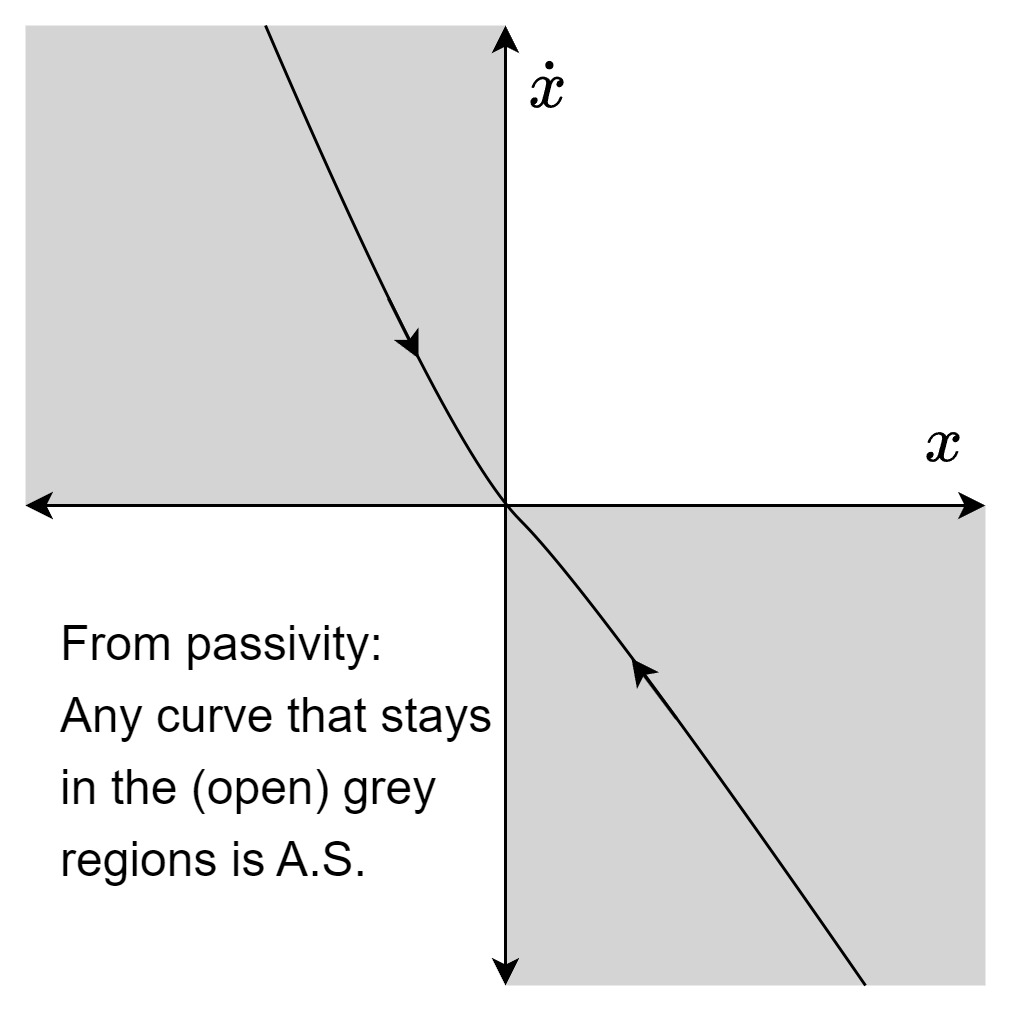
\includegraphics[width=0.5\linewidth]{figures/passivity_plot.jpg}
    % \caption{Caption}
    % \label{fig:enter-label}
\end{figure}



%% 
\subsection*{Region of Attraction Process}
Given the system \(\dot{x} = f(x)\), linearize to find \(A\), and recast as 
\begin{equation*}
    \dot{x}= (A + G(x)) x = f(x) 
\end{equation*}
\begin{enumerate}
    \item Introduce Lyapunov candidate function 
    \begin{align*}
        \vofx &= x^TPx,\, P \succ 0 \\
        \vdotofx &= -x^TQx + 2x^TPG(x)
    \end{align*}
    where \(Q \succ 0\) satisfies the Lyapunov equation~\eqref{eq:lyapunov_eq}.

    \item Find the region where \(\vdotofx \prec 0\) for A.S. or \(\vdotofx < -k_3\|x\|^a\) for E.S. To analyze, apply norms
    \begin{align*}
        \vdotofx & \leq -x^TQx + 2\|x\| \|PG(x)\|\\
        & \leq -\lambda_{\min} (Q) \|x\|^2 + 2\|x\| \|PG(x)\|\\
        & \leq -(1-K)\lambda_{\min} (Q)\|x\|^2 + 2\|x\| \|PG(x)\| - K\lambda_{\min} (Q) \|x\|^2\\
        & \leq \underbrace{-k_3 \|x\|^2}_{\text{for E.S}} + \underbrace{2\|x\| \|PG(x)\| - K\lambda_{\min} (Q) \|x\|^2}_{\text{for ROA}}
    \end{align*}
    where \(K\in(0,\,1)\) is chosen iteratively to achieve desired ROA-speed tradeoff.

    \item Towards E.S. (Thm 3.6) find \(K\) such that the ROA term \(\leq0\), and the following provides a quadratic surface as a lower estimate. (\(K=0\) provides a quadratic upper surface as an estimate.) 
    \begin{equation*}
        \vdotofx \leq -(1-K)\lambda_{\min}(Q) \|x\| < 0 
    \end{equation*}

    \item As domain \(D\) is becoming more and more constrained throughout this process, use \(D\) to characterize where \(\vdotofx \prec 0\) (within the ball). Using such a location, find the value of the level set \(\vofx = c\), and construct \(\Omega_c = \{ x \in \mathds{R}^n | \vofx < c\}\). If \(\vofx \succ 0\), and \(\vdotofx \prec 0\) in \(\Omega_c\), then the ROA is A.S.

    \item For E.S., use the constructed bounds on \(\vofx\), and determine bounds on \(\vdotofx\) by finding values \(k_1,\, k_2,\) and \(k_3\) to satisfy Thm~3.6 USING NORMS. 
    \begin{equation*}
        \longrightarrow \lambda_{\min} (P) \|x\|^2 \leq x^TPx \leq \lambda_{\max}(P) \|x\|^2 \longleftarrow
    \end{equation*}
    Note, small \(K\) results in faster \(\tau\), but smaller ROA, and vice-versa for big \(K\). Start with \(K=0.5\), and adjust based upon resulting system behavior until happy.

    \item As the ROA term might be difficult to ascertain (mentally or computationally), it is helpful to describe an open ball within the ROA (\(B_r = \{x \in \mathds{R}^n |\, \|x\| < r\} \subset \Omega_c\)). Use the defined \(\Omega_c\) bounds OR norms of \(P\) formulation of \(\vofx\) to determine \(r\). Note: the ball may vary in size depending on how conservative the bounding is (\textit{i.e.}, bounding above vs below, etc).
\end{enumerate}

%%
\subsection*{Standard Forms}
\subsubsection*{Normal Form}
Uses \(z =T(x)\) to convert system to 
\begin{align*}
    \dot{\eta} =& f_0(\eta,\, \xi)\\
    \dot{\xi} =& A_c\xi + B_c \left[L_f^\rho h(x) + L_g^{\rho-1}L_f h (x)u\right]\\
    y =& C_c\xi
\end{align*}
\subsubsection*{Controller Form}
If \(\rho=n\), normal form is equivalent to controller form
\begin{align*}
    \dot{x} = Ax + B[\psi(x) + \gamma(x)u]
\end{align*}
\subsubsection*{Observer Form}
\begin{align*}
    \dot{\hat{x}} = A\hat{x} + \psi(u,\,y) + H(y-C\hat{x}) = \hat{f}(\hat{x}) + H(y - C\hat{x})
\end{align*}


%%
\subsection*{Control}
\subsubsection*{Linearization}
Given \(\dot{x} =f(x,\,u)\), linearize to find \(\dot{x} \approx Ax + Bu\) where
\begin{equation*}
    A = \left. \frac{\partial f}{\partial x}\right|_{\overline{x},\, \overline{u}} \hspace{30pt} B = \left. \frac{\partial f}{\partial u}\right|_{\overline{x},\, \overline{u}} 
\end{equation*}
and the pair \((A,\,B)\) must be controllable, or stabilizable (the zero dynamics are minimum phase). Choose \(u_{fb} = - Kx\) where \(K\in \mathds{R}^n\) are such that \((A-BK)\) is Hurwitz, etc.  Then, assemble \(u = u_{ss} + u_{fb}\) where \(u_{ss}\) is the input that keeps the system at \(x =\overline{x}\). Note: If \(K=K(\text{something})\), this is gain scheduling.


%%
\subsubsection*{Feedback Linearization}
Considering the system \(\dot{x} = f(x) + G(x)u\), with \(f(0) = 0\), \(x\in\mathds{R}^n\), and \(u\in\mathds{R}^m\), transform to controller form using \(z=T(x)\). If the pair \((A,\,B)\) is controllable, and \(\gamma(x)\) is nonsingular on some \(D \subset \mathds{R}^n\), then choose 
\begin{equation*}
    u = \gamma^{-1}(x) \left[ -\psi(x) - Kz\right]
\end{equation*}
which results in \(\dot{z} = (A-BK)z\), and design \(K\) for Hurwitz, etc. 

Note: While \(z\) is guaranteed(designed) to be exponentially stable, \(x\) is only guaranteed to be asymptotically stable, as stability type is not kept through \(x = T^{-1}(z)\). 


\subsubsection*{Partial Feedback Linearization}
If relative degree \(\rho < n\), transform the system into normal form. If the pair \((A,\,B)\) is controllable, \(f_0(0) =0\) (\textit{i.e.}, \(\overline{\eta} =0\) is an equilibrium point), \(\psi(0) = 0\), and \(\dot{\eta}(\eta, \,\xi=0)\) is A.S., choose 
\begin{equation*}
    u = \gamma^{-1}(x) \left[-\psi(x) -K\xi\right]
\end{equation*}
with \(K\) designed for Hurwitz, etc. and the uncontrolled states \(\eta\) are stable on their own (\textit{i.e.}, system is min. phase).



%%
\subsubsection*{Backstepping}
The idea is to steer the controllable states \(\xi\) in such a way that the uncontrollable states \(\eta\) behave as desired. Given \(\dot{x} = f(x) + G(x)u\), transform the system into 
\begin{align*}
    \dot{\eta} =& f_a(\eta) + g_a(\eta)\xi\\
    \dot{\xi} =& f_b(\eta,\,\xi) + g_b(\eta,\,\xi)u
\end{align*}
\underline{Technique}:
\begin{enumerate}
    \item Treat \(\xi\) as the input into \(\dot{\eta}\) equation and design \(\xi = \phi(\eta)\) to stabilize \(\eta \to \eta_{\text{des}}\), with the desired stability characteristics
    \begin{equation*}
        \dot{\eta} = f_a(\eta) + g_a(\eta)\phi(\eta)
    \end{equation*}
    Choose \(V_a(\eta) \succ 0\) such that
    \begin{equation*}
        \dot{V}_a(\eta) = \frac{\partial V_a}{\partial \eta} \frac{d \eta}{dt} =  \frac{\partial V_a}{\partial \eta} \left[f_a(\eta) + g_a(\eta)\phi(\eta) \right] \preceq -W(\eta)
    \end{equation*}
    where \(\phi(\eta)\) is constructed such that \(W(\eta) \succ 0\).
    
    \item Derive control input \(u\) to satisfy step 1, and to drive \(\xi \to \xi_{\text{des}}\). Apply \(\xi=\phi(\eta)\) to system
    \begin{equation*}
        \dot{\eta} = \underbrace{f_a(\eta) + g_a(\eta)\phi(\eta)}_{\text{A.S./E.S. by design}} +  \underbrace{g_a(\eta) [\xi -\phi(\eta)]}_{\text{drive } \xi \to \phi(\eta) \text{ to make this zero}}
    \end{equation*}
    The second  term acts a disturbance until equality holds, and results in undesired dynamics until satisfied. Define error \(z = \xi - \phi(\eta)\) and analyze its dynamics to ensure/guarantee stability.     
    \begin{align*}
        \dot{\eta} =& f_a(\eta) + g_a(\eta)\phi(\eta) + g_a(\eta)z\\
        \dot{z} =& \dot{\xi} - \frac{\partial \phi}{\partial \eta} \frac{d\eta}{dt}\\
        =& f_b(\eta,\, \xi) + g_b(\eta,\,\xi) u \\
        &-\frac{\partial \phi}{\partial \eta} \left[f_a(\eta) + g_a(\eta)\phi(\eta) + g_a(\eta)z \right]\\
        =& F(\eta,\,\xi) + g_b(\eta,\,\xi)u
    \end{align*}
    Define \(V_b(\eta,\,z) = V_a(\eta) + \frac{1}{2}z^2\), and 
    \begin{align*}
        \dot{V}_b(\eta,\,z)  =&  \frac{\partial V_a}{\partial \eta} \left[f_a(\eta) + g_a(\eta)\phi(\eta) \right]  \hspace{10pt}\\
        &+ z\left[ F(\eta,\,\xi) + \frac{\partial V_a}{\partial \eta} g_a(\eta) + g_b(\eta,\,\xi) u\right] 
    \end{align*}
    where the first term is \(\preceq -W(\eta)\) and \(u\) is designed such that \(\dot{V}_b(\eta,\,z) \prec 0\). Using feedback linearization
    \begin{equation*}
        u = g_b^{-1} (\eta,\,\xi) \left[- F(\eta,\,\xi) - \frac{\partial V_a}{\partial \eta} g_a(\eta) - k_zz \right]
    \end{equation*}
    and the origin \((\eta=0,\, \xi=0)\) is A.S. If \(z\to 0\), then \(\eta\to0\), and if \(\xi=\phi(\eta=0)\) then \(\xi\to0\). 
\end{enumerate}
Backstepping can be applied recursively (see 11/5/24), or each layer can be robusted by accounting for model uncertainty by adding SMC.

\subsubsection*{Sliding Mode Control}
This controller is demonstrated by example. Consider
\begin{align*}
    \dot{x}_1 =& x_2\\ \dot{x}_2=& h(x) + g(x) u
\end{align*}
where the system is locally Lipschitz to equilibrium point \(\overline{x} =0\), and \(g(x) \geq g_0>0\). As in backstepping, let \(x_2 = -ax_1\) with \(a>0\) so that 
\begin{equation*}
    \dot{x}_1 = -x_1 
\end{equation*}
is an E.S. first order system, with \(a\) chosen for desired dynamics. Now, design a controller to drive \(x_2 \to  -ax_1\), and ensure stability of the system. Describe surface
\begin{equation*}
    s   = x_2 -\phi(x)= x_2 + ax_1
\end{equation*}
such that if \(x_1 \to0\) then \(\phi(0) = x_2 =0\). Let \(V(s) = \frac{1}{2}s^2 \succ 0\) and 
\begin{align*}
    \dot{V}(s) =& s\dot{s} = s(\dot{x}_2+a\dot{x}_1)\\
    =& s(ax_2 + h(x)) + sg(x)u\\
    =& s g(x) \left(\frac{ax_2 + h(x)}{g(x)}\right) + sg(x)u\\
    \leq& |s|g(x) \left| \frac{ax_2 + h(x)}{g(x)} \right| + sg(x)u
\end{align*}
Define \(\rho(x)\) to be model-based, by considering the absolute values of each entry, or hammer based, by considering largest possible everything so \(\rho(x) =\) const.
\begin{equation*}
    \rho(x) \geq \left| \frac{ax_2 + h(x)}{g(x)} \right| \geq 0
\end{equation*}
Then design \(u\) for this all to be n.s.d.
\begin{equation*}
    \dot{V}(s) \leq |s|g(x) \rho(x) + sg(x)u \preceq 0
\end{equation*}
Let
\begin{equation*}
    u = -\beta(x) \operatorname{sat}(s/\varepsilon_s) \hspace{30pt} \varepsilon_s \in \mathds{R}_{++} \text{ tuned for chatter}
\end{equation*}
\begin{equation*}
    \beta(x) = \rho(x) + \beta_0 \hspace{30pt} \beta_0 \in \mathds{R}_{++} \text{ tuned for robustness}
\end{equation*}
This results in a practically stabilized system.



%%
\subsubsection*{Lyapunov Redesign}
When there exists a satisfactory controller, and robustness is desired. Consider the system with model uncertainty acting as an input disturbance \(\delta\)
\begin{equation*}
    \dot{x} = f(x) + G(x) \left[u+ \delta(x,\,t,\,u)\right]
\end{equation*}
where the nominal controller \(u = \phi(x)\) achieves
\begin{align*}
    V(x) =& \succ0 \\
    \dot{V}(x) =& \frac{\partial  V}{\partial x}\left[ f(x) + G(x)\phi(x) \right] \preceq -W(x) \prec 0
\end{align*}
with no uncertainty present. To account for uncertainty, adjust control input to \(u = \phi(x) + v\), where \(v\) deals with the effects of uncertainty. To do this, uncertainty \(\delta\) is manipulated to satisfy 
\begin{equation*}
    \|\delta(x,\, t,\, u) \| \leq \rho(x) + \kappa_0\|v\|
\end{equation*}
Applying to the system gives
\begin{equation*}
    \dot{x} = \underbrace{f(x) + G(x)\phi(x)}_{\text{nominal}}  + G(x)\left[ v+ \delta\right]
\end{equation*}
and \(v\) is designed to achieve \(\dot{V}(x)\preceq0\)
\begin{align*}
    \dot{V}(x) =& \frac{\partial V}{\partial x} \left[f(x) + G(x)\phi(x) \right] + \frac{\partial V}{\partial x}G(x)(v+\delta)\\
    \leq& -W(x) + \omega^Tv + \omega^T\delta, \hspace{20pt} \omega^T:= \frac{\partial V}{\partial x}G(x)
\end{align*}
\begin{align*}
    \omega^Tv + \omega^T\delta \leq& \omega^Tv + \|\omega^T\| \|\delta\|\\
    \leq& \omega^Tv + \|\omega\| (\rho(x) + \kappa_0\|v\|)
\end{align*}
Choose input \(v\) to achieve A.S., let
\begin{equation*}
    v = -\beta(x) \operatorname{sat}\left( \frac{\beta(x) \|\omega\|}{\mu}\right) \hspace{20pt} \mu \in \mathds{R}_{++} \text{ tuned for chatter}
\end{equation*}
where \(\beta(x) \geq \rho(x)/(1-\kappa_0)\). This results in a practically stabilized system.



%%
\subsection*{Observers}
All observers define error dynamics by the following, where hat indicates nominal parameters and observed states
\begin{equation*}
    \Tilde{x} := x - \hat{x} \hspace{30pt} \Longrightarrow \hspace{30pt} \dot{\Tilde{x}} = \dot{x} - \dot{\hat{x}}
\end{equation*}
\subsubsection*{Linear (local) Observer}
Consider
\begin{align*}
    \dot{x} =& f(x,\,u)\\
    y =& h(x)
\end{align*}
Define observer
\begin{equation*}
    \dot{\hat{x}} = \hat{f} ( \hat{x},\,u)  + H (h(x) - h(\hat{x})) \hspace{30pt} H\in\mathds{R}^n
\end{equation*}
The error dynamics are linearized (\(f \approx \hat{f}\)) by
\begin{align*}
    \dot{\Tilde{x}} =& f(x,\,u) - \hat{f}(\hat{x},\, u) + H (h(x) - h(\hat{x}))\\
     \approx & \left.\frac{\partial f}{\partial x}\right|_{\overline{x},\,\overline{u}} x - \left.\frac{\partial \hat{f}}{\partial x}\right|_{\overline{x},\,\overline{u}}\hat{x} + HC \left.\frac{\partial h(x)}{\partial x}\right|_{\overline{x},\,\overline{u}}(x-\hat{x})\\
     \approx & (A+HC)\Tilde{x}
\end{align*}
Then design \(H\) for Hurwitz, and desired error dynamics (fast as or faster than state dynamics)


\subsubsection*{High Gain Observer}
This is one flavor of many. Consider 
\begin{align*}
    \dot{x} = & Ax + g(y,\,u)\\
    y =& Cx
\end{align*}
Define observer
\begin{equation*}
    \dot{\hat{x}} = A \hat{x} + \hat{g}(y,\,u) + H (y-C\hat{x}) \hspace{30pt} H \in\mathds{R}^n
\end{equation*}
The error dynamics are
\begin{equation*}
    \dot{\Tilde{x}} = (A-HC) \Tilde{x} + \underbrace{g(y,\,u) - \hat{g}(y,\,u)}_{\text{uncertainty may cause } \Tilde{x}_{ss} \neq0}
\end{equation*}
Let \(\delta(x,\,\hat{x}) :=g(y,\,u) - \hat{g}(y,\,u)\), act as the input to the system, and convert to transfer function form using \(y = (sI - A + HC)^{-1}B\delta\). Bop it with the final value theorem
\begin{equation*}
    \lim_{t\to\infty} f(t) = \lim_{s\to 0 } sF(s)
\end{equation*}
to determine the relative sizings of \(h_i\) (\textit{e.g.}, \(h_2 >>h_1 >>1\) resulting in \(h_1 = \alpha_1/\varepsilon_o\), \(h_2 = \alpha_2/\varepsilon^2_o\), where \(\alpha_1,\,\alpha_2\) are chosen for desired dynamics).




\subsubsection*{Global Observer}
Convert to the general form
\begin{align*}
    \dot{x} =& Ax + \psi(y,\,u) + \phi(x,\,u)\\
    y =&Cx
\end{align*}
Ensure that the pair \((A,\,C)\) is observable, \(\phi(x,\,u)\) is locally Lipschitz with coefficient \(L\) satisfying
\begin{equation*}
    \|\phi(x,\,u) - \phi(z,\,u)\| \leq L \|x-z\|
\end{equation*}
Define observer 
\begin{equation*}
    \dot{\hat{x}} = A\hat{x} + \psi(y,\,u) + \phi(\hat{x},\,u) + H(y-C\hat{x}) \hspace{30pt} H\in\mathds{R}^n
\end{equation*}
The \(\psi\) equation contains known quantities that cancel out in the next step, whereas the \(\phi\) equation contains uncertain quantities. The error dynamics are
\begin{equation*}
    \dot{\Tilde{x}} = (A-HC) \Tilde{x} + \underbrace{\phi(x,\,u) - \hat{\phi}(\hat{x},\,u)}_{\text{disturbance due to uncertainty}}
\end{equation*}
Choosing \(Q\succ0\) to satisfy Eq.~\eqref{eq:lyapunov_eq}, via lyap(), \(P\succ0\) is found and Lyapunov function formed
\begin{align*}
    V(\Tilde{x}) =& \Tilde{x}^TP\Tilde{x}\\
    \dot{V}(\Tilde{x})=&  -\Tilde{x}^TQ\Tilde{x} + 2\Tilde{x}^TP[\phi(x,\,u) - \hat{\phi}(\hat{x},\,u)]\\
    \leq& -\|\Tilde{x}\|^2 + 2L\|P\|\, \|\Tilde{x}\|^2\\
    \leq& -\|\Tilde{x}\|^2 (1-2L\|P\|)
\end{align*}
Then \(\dot{V}(\Tilde{x}) \preceq 0\) if \(2L\|P\| <1\), and error dynamics are A.S.



%%
\subsection*{Output Feedback Control}
\subsubsection*{Linearization}
Given \(\dot{x} = f(x,\,u)\), \(y=h(x)\) linearize as such
\begin{equation*}
    A = \left.\frac{\partial f}{\partial x}\right|_{\overline{x},\,\overline{u}} \hspace{15pt}  B = \left.\frac{\partial f}{\partial x}\right|_{\overline{u},\,\overline{u}} \hspace{15pt}  C = \left.\frac{\partial h}{\partial x}\right|_{\overline{x},\,\overline{u}} \hspace{15pt}  D = \left.\frac{\partial h}{\partial u}\right|_{\overline{x},\,\overline{u}} \hspace{15pt}
\end{equation*}
where pairs \((A,\,C)\) and \((A,\,B)\) are detectable and stabilizable, respectively. Convert to the general output feedback form
\begin{align*}
    \dot{z} =& Fz + Gy\\
    u =& Lz + My
\end{align*}
where \(z\) are the observer states, \(y\) is the sensor output, \(u\) is control based on \(z,\,y\). Combine this with the system to achieve
\begin{equation*}
    \begin{bmatrix}
        \dot{x} \\ \dot{z} 
    \end{bmatrix} = \begin{bmatrix}
        A+BMC & BL \\ GC & F
    \end{bmatrix} \begin{bmatrix}
        x \\ z
    \end{bmatrix}
\end{equation*}
Introducing an observer with \(\hat{x}:= z\), \(F:= (A-BK-HC)\), \(G:=H\), \(K:=-L\), and \(M:=0\) gives
\begin{equation*}
    \begin{bmatrix}
        \dot{x} \\ \dot{\hat{x}}
    \end{bmatrix} = \begin{bmatrix}
        A & -BK\\ HC & A-BK-HC
    \end{bmatrix}\begin{bmatrix}
        x\\ \hat{x}
    \end{bmatrix}
\end{equation*}
which is what runs real-time. This is still coupled and hard to design. Converting once more with error defined \(\Tilde{x} := x -\hat{x}\) gives the decoupled system, which is tractable for design.
\begin{equation*}
    \begin{bmatrix}
        \dot{x} \\ \dot{\Tilde{x}}
    \end{bmatrix} = \begin{bmatrix}
        A-BK & BK \\ 0 & A-HC
    \end{bmatrix} \begin{bmatrix}
        x\\ \tilde{x}
    \end{bmatrix}
\end{equation*}



%%
\subsection*{Tracking Control}
Consider \(\dot{x} = f(x,\,u)\), and put it into the form
\begin{align*}
    \dot{\eta} =& f_0(\eta,\,\xi)\\
    \dot{\xi}_1 = & \xi_2\\
    & \vdots\\
    \dot{\xi}_\rho =& a(\eta,\,\xi) + b(\eta,\,\xi) u\\
    y=& x_1
\end{align*}
where \(b(\eta,\xi) \geq b_0 > 0\), and the system is minimum phase. The goal is to drive \(y(t) \to y_r(t) := r(t)\). Define error as 
\begin{align*}
    e_1 =& \xi_1 - r(t)\\
    e_2 =& \xi_2 - \dot{r}(t)\\
    & \vdots\\
    e_\rho =& \xi_\rho - r^{(\rho-1)}(t)
\end{align*}
with dynamics
\begin{align*}
    \dot{e}_1 =& e_2\\    
    & \vdots\\
    \dot{e}_\rho =& a(\eta,\,\xi) + b(\eta,\,\xi)u - r^{(\rho)}(t)
\end{align*}
\begin{equation*}
    \dot{e} = A_c e + B_c\left[ a(\eta,\,\xi) + b(\eta,\,\xi)u - r^{(\rho)}(t)\right]
\end{equation*}
Do feedback linearization by choosing input 
\begin{equation*}
    u = b^{-1}(\eta,\,\xi) \left[-a(\eta,\,\xi) + r^{(\rho)}(t) + v\right] \hspace{30pt} v = Ke
\end{equation*}
resulting in \(\dot{e} = (A_c + B_cK) e\) Where \(K\) is designed for Hurwitz, etc.


\subsubsection*{Robust Tracking Control}
Assume form
\begin{align*}
    \dot{\eta} =& f_0(\eta,\,\xi)\\
    \dot{e}_i =& e_{i+1} \hspace{30pt} 1 \leq i < \rho\\
    \dot{e}_\rho =& a(\eta,\,\xi) + b(\eta,\,\xi)u - r^{(\rho)}(t) + \delta(t,\,\eta,\,\xi,\,u)
\end{align*}
Define sliding manifold dynamics
\begin{align*}
    s := e_\rho + \sum_{i=1}^{\rho-1} k_ie_i \hspace{30pt} \dot{s} = \dot{e}_\rho  + \sum_{i=1}^{\rho-1} k_ie_{i+1}
\end{align*}
where \(K\) are chosen using characteristic equation 
\begin{equation*}
    \lambda^{\rho-1} + k_{\rho-1}\lambda^{\rho-2} + \dots + k_1 = 0
\end{equation*}
Based upon \(\dot{e}_\rho\), and nominal values \(\hat{a}\), and \(\hat{b}\), let input 
\begin{equation*}
    u = \hat{b}^{-1}(\eta,\,\xi) \left[ -\hat{a}(\eta,\,\xi) + r^{(\rho)}(t) - \sum_{i=1}^{\rho-1} k_ie_{i+1}\right] + v
\end{equation*}
be applied into \(\dot{s}\)
\begin{equation*}
    \dot{s} = b(\eta,\,\xi)v + \Delta(t,\,\eta,\,\xi,\,v)
\end{equation*}
Using \(V(s) = \frac{1}{2}s^2\), find \(v\) such that \(\dot{V}(s) \prec 0\), using the typical SMC design flow
\begin{equation*}
    \left| \frac{\Delta(t,\,\eta,\,\xi,\,v)}{b(\eta,\,\xi)}\right| \leq \overline{\rho}(\eta,\,\xi)  + \kappa_0\|v\|
\end{equation*}
\begin{equation*}
    v = - \beta(\eta,\,\xi) \operatorname{sat}(s/\varepsilon_s) \hspace{30pt} \varepsilon_s\in\mathds{R}_{++} \text{ tuned for chatter}
\end{equation*}
\begin{equation*}
    \beta(\eta,\,\xi) \geq \overline{\rho}(\eta,\,\xi) \frac{1}{1-\kappa_0} + \beta_0 \hspace{30pt} \beta_0\in\mathds{R}_{++} \text{ tuned for robustness}
\end{equation*}



%%
\subsection*{Notes}
\begin{itemize}
    \item In choosing a Lyapunov function, pick \(\vofx\) that generates a level curve such that it ``matches'' phase portrait in shape, \textit{e.g.} a circular \(\vofx\) would poorly  a phase portrait with elliptical level sets.

    \item An equilibrium point \(\eqpt\) is \emph{hyperbolic} if it has NO eigenvalues on the imaginary axis[citation needed].
\end{itemize}


% \newpage
% \vspace{2in}
\begin{center}
    All theorems, lemmas, and quotes are taken from Nonlinear Controls 3rd edition by Hassan Khalil.
\end{center}

\end{document}